\documentclass[aspectratio=169,11pt]{beamer}

% ============================================================
% THEME & COLOURS (matched to GDP PowerPoint)
% ============================================================
\usetheme{default}
\usecolortheme{default}
\setbeamertemplate{navigation symbols}{}

\definecolor{gdpPurple}{HTML}{633E88}
\definecolor{gdpDarkBlue}{HTML}{0C406D}
\definecolor{gdpNavy}{HTML}{091932}
\definecolor{gdpOrange}{HTML}{DD7A0F}
\definecolor{gdpSlate}{HTML}{3B4950}
\definecolor{gdpLightGray}{HTML}{E7E6E6}
\definecolor{gdpBurgundy}{HTML}{820E21}

\setbeamercolor{background canvas}{bg=white}
\setbeamercolor{normal text}{fg=gdpSlate}
\setbeamercolor{frametitle}{fg=gdpPurple,bg=white}
\setbeamercolor{framesubtitle}{fg=gdpDarkBlue,bg=white}
\setbeamercolor{title}{fg=gdpPurple}
\setbeamercolor{subtitle}{fg=gdpDarkBlue}
\setbeamercolor{author}{fg=gdpSlate}
\setbeamercolor{institute}{fg=gdpSlate}
\setbeamercolor{date}{fg=gdpSlate}
\setbeamercolor{item}{fg=gdpDarkBlue}
\setbeamercolor{subitem}{fg=gdpPurple}
\setbeamercolor{block title}{fg=white,bg=gdpDarkBlue}
\setbeamercolor{block body}{fg=gdpSlate,bg=gdpLightGray!30}
\setbeamercolor{block title alerted}{fg=white,bg=gdpBurgundy}
\setbeamercolor{block body alerted}{fg=gdpSlate,bg=gdpLightGray!30}
\setbeamercolor{footline}{fg=gdpSlate}
\setbeamercolor{headline}{fg=white,bg=gdpPurple}

\usepackage{helvet}
\renewcommand{\familydefault}{\sfdefault}
\usepackage{amsmath,amssymb,graphicx,booktabs,array}
\usepackage{pifont}
\newcommand{\cmark}{\ding{51}}
\newcommand{\xmark}{\ding{55}}

\setlength{\tabcolsep}{3pt}
\setbeamertemplate{itemize/enumerate body begin}{\small}
\setbeamertemplate{itemize/enumerate subbody begin}{\footnotesize}
\addtolength{\leftmargini}{-0.3cm}
\addtolength{\leftmarginii}{-0.2cm}

\setbeamertemplate{frametitle}{%
  \vspace{0.2cm}
  \textbf{\large\insertframetitle}
  \vspace{0.05cm}
  \par\textcolor{gdpDarkBlue}{\rule{\textwidth}{1.2pt}}
  \vspace{-0.3cm}
}

\setbeamertemplate{footline}{%
  \leavevmode%
  \hbox{%
    \begin{beamercolorbox}[wd=.333\paperwidth,ht=2.5ex,dp=1ex,leftskip=0.3cm]{footline}%
      \insertshortauthor
    \end{beamercolorbox}%
    \begin{beamercolorbox}[wd=.333\paperwidth,ht=2.5ex,dp=1ex,center]{footline}%
      \insertshorttitle
    \end{beamercolorbox}%
    \begin{beamercolorbox}[wd=.333\paperwidth,ht=2.5ex,dp=1ex,rightskip=0.3cm]{footline}%
      \insertframenumber{}
    \end{beamercolorbox}%
  }%
}

\setbeamertemplate{title page}{
  \vspace{1.5cm}
  \begin{center}
    {\Huge\bfseries\textcolor{gdpPurple}{\inserttitle}}\\[0.4cm]
    {\Large\textcolor{gdpDarkBlue}{\insertsubtitle}}\\[1.2cm]
    {\large\textcolor{gdpSlate}{\insertauthor}}\\[0.3cm]
    {\normalsize\textcolor{gdpSlate}{\insertinstitute}}\\[0.3cm]
    {\normalsize\textcolor{gdpSlate}{\insertdate}}
  \end{center}
}

\title{Continuous Analog Wave Computation in Porous Media}
\subtitle{Progress Update -- Methodology, Model Validity and Current Explorations}
\author{S. Venugopal}
\institute{Cranfield University\hspace{0.3cm}|\hspace{0.3cm}Supervisors: Prof. Weisi Guo, Prof. Takis Tsoutsanis}
\date{23 June 2026}

\begin{document}

\begin{frame}[plain]
  \titlepage
\end{frame}

% ============================================================
\begin{frame}{Aim and Research Question}
  \textbf{Core aim:} Treat a structured acoustic medium as a trainable physical neural-network layer.

  \vspace{0.4cm}
  \textbf{Research questions:}
  \begin{enumerate}
    \item Can a passive porous acoustic medium implement a trainable transformation?
    \item What physical constraints limit the class of operations it can perform?
    \item Can we go beyond non-negative weights using phase-encoded readout?
    \item What physical nonlinearity could replace a digital activation function?
  \end{enumerate}

  \vspace{0.3cm}
  \textcolor{gdpSlate}{\small The project focuses on the simulation framework; experimental realisation is future work.}
\end{frame}

% ============================================================
\begin{frame}{Literature Positioning}
  \begin{columns}[T]
    \begin{column}{0.32\textwidth}
      \textbf{Hughes et al. 2019}\\[0.1cm]
      \footnotesize
      Wave physics as an analog recurrent neural network.
      \begin{itemize}
        \item First demonstration that a wave system can be trained like an RNN.
        \item Uses an intensity-dependent wave speed as nonlinearity.
      \end{itemize}
    \end{column}
    \begin{column}{0.32\textwidth}
      \textbf{Kalthoff et al. 2025}\\[0.1cm]
      \footnotesize
      Acoustic neural networks under physical constraints.
      \begin{itemize}
        \item Signals and weights must be non-negative.
        \item Constrained architectures still classify well.
      \end{itemize}
    \end{column}
    \begin{column}{0.32\textwidth}
      \textbf{This project}\\[0.1cm]
      \footnotesize
      Probe the boundary of what is physically possible.
      \begin{itemize}
        \item Porous-medium substrate.
        \item Signed weights via phase.
        \item Physical nonlinearities.
      \end{itemize}
    \end{column}
  \end{columns}

  \vspace{0.4cm}
  \begin{center}
    \textcolor{gdpDarkBlue}{\textbf{Hughes = existence proof \quad $\rightarrow$ \quad Kalthoff = design rules \quad $\rightarrow$ \quad This work = push the boundary}}
  \end{center}
\end{frame}

% ============================================================
\begin{frame}{Domain Description}
  \begin{columns}[T]
    \begin{column}{0.55\textwidth}
      \textbf{2-D acoustic domain}
      \begin{itemize}
        \item Square domain with absorbing/sponge boundaries.
        \item Input sources on the left (line sources, different $y$).
        \item Output probes on the right (different $y$).
        \item Design region in the centre.
        \item Coarse design grid mapped smoothly to the FDTD grid.
      \end{itemize}

      \vspace{0.2cm}
      \textbf{Design variables}
      \begin{itemize}
        \item Local sound speed $c(x,y)$, or
        \item Porous-medium parameters: $\phi$, $\sigma$, $\alpha_\infty$.
      \end{itemize}
    \end{column}
    \begin{column}{0.43\textwidth}
      \centering
      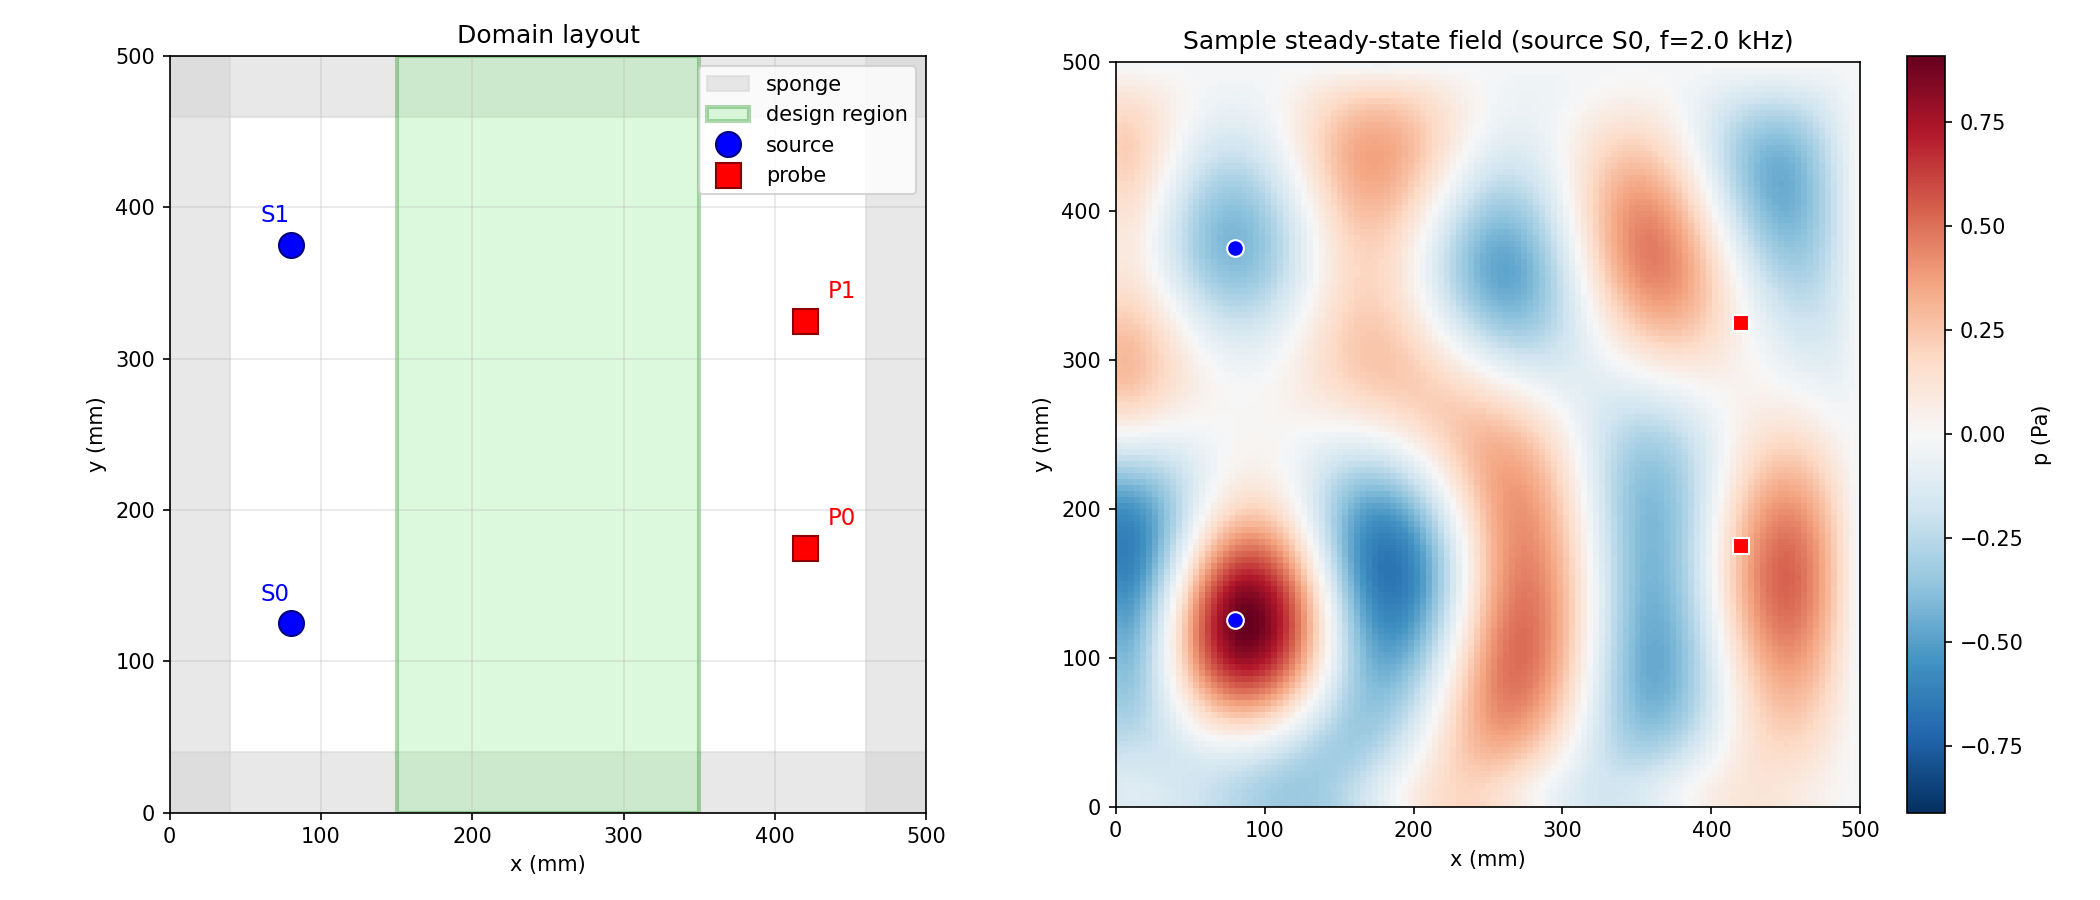
\includegraphics[width=\textwidth]{../Analysis/figures/fdtd_zk_setup_diagram.png}
      \\[0.1cm]
      {\footnotesize Example domain layout and sample field.}
    \end{column}
  \end{columns}
\end{frame}

% ============================================================
\begin{frame}{Governing Equations}
  \small
  \textbf{Frequency-domain Helmholtz equation with spatially varying JCA coefficients}
  \begin{align*}
    \nabla \cdot \left( \frac{1}{\tilde{\rho}(\omega, \mathbf{x})} \nabla p \right) + \frac{\omega^2}{\tilde{K}(\omega, \mathbf{x})} \, p = S(\omega) \, \delta(\mathbf{x} - \mathbf{x}_s)
  \end{align*}

  \vspace{0.2cm}
  \textbf{Effective properties are complex, frequency-dependent, and spatially varying:}
  \begin{align*}
    \tilde{\rho}(\omega, \mathbf{x}) &= \frac{\rho_0 \, \tilde{\alpha}(\omega, \mathbf{x})}{\phi(\mathbf{x})} \\
    \tilde{K}(\omega, \mathbf{x}) &= \frac{\gamma P_0}{\phi(\mathbf{x})} \left[ \gamma - \frac{\gamma - 1}{1 + \frac{8 \eta}{j \omega \rho_0 Pr \Lambda'(\mathbf{x})^2} \sqrt{1 + j \frac{\omega \rho_0 Pr \Lambda'(\mathbf{x})^2}{16 \eta}}} \right]^{-1}
  \end{align*}

  \vspace{0.2cm}
  \footnotesize
  \begin{tabular}{llllll}
    $p$ & pressure & $\mathbf{x}$ & position & $\omega$ & angular frequency \\
    $\phi$ & porosity & $\sigma$ & flow resistivity & $\alpha_\infty$ & high-frequency tortuosity \\
    $\Lambda$ & viscous length & $\Lambda'$ & thermal length & $Pr$ & Prandtl number
  \end{tabular}
\end{frame}

% ============================================================
\begin{frame}{Constitutive Relations}
  \small
  \textbf{JCA dynamic tortuosity (viscous losses)}
  \begin{align*}
    \tilde{\alpha}(\omega, \mathbf{x}) = \alpha_\infty(\mathbf{x}) \left[
      1 + \frac{\sigma(\mathbf{x}) \phi(\mathbf{x})}{j \omega \rho_0 \alpha_\infty(\mathbf{x})}
      \sqrt{1 + j \, \frac{4 \alpha_\infty(\mathbf{x})^2 \eta \rho_0 \omega}{\sigma(\mathbf{x})^2 \phi(\mathbf{x})^2 \Lambda(\mathbf{x})^2}}
    \right]
  \end{align*}

  \vspace{0.2cm}
  \textbf{What it means physically}
  \begin{itemize}
    \item $\alpha_\infty(\mathbf{x})$ is the geometric high-frequency tortuosity.
    \item $\tilde{\alpha}(\omega, \mathbf{x})$ captures the viscous boundary-layer transition from low to high frequency.
    \item $\tilde{\rho}(\omega, \mathbf{x}) = \rho_0 \tilde{\alpha}(\omega, \mathbf{x}) / \phi(\mathbf{x})$.
  \end{itemize}

  \vspace{0.2cm}
  \textcolor{gdpBurgundy}{\textbf{Caveat:} The low-frequency ZK model replaces $\tilde{\alpha}(\omega, \mathbf{x})$ by $\alpha_\infty(\mathbf{x})$. At 2 kHz with typical foams ($\Lambda \sim 100$~$\mu$m), $Wo \sim 3$, so the full frequency-dependent JCA form is the physically correct target.}
\end{frame}

% ============================================================
\begin{frame}{Methodology Pipeline}
  \begin{center}
    \small
    \begin{tabular}{ccccccc}
      \textbf{Design grid} & $\to$ & \textbf{Material map} & $\to$ & \textbf{FDTD} & $\to$ & \textbf{Readout} \\[0.15cm]
      $\phi, \sigma, \alpha_\infty$ per block & & Smooth interpolation & & Wave propagation & & Complex amplitude \\[0.4cm]
      \textbf{Loss} & $\to$ & \textbf{Optimiser} \\[0.15cm]
      $\|W_\text{eff} - W_\text{target}\|$ & & Differential evolution
    \end{tabular}
  \end{center}

  \vspace{0.4cm}
  \textbf{Key point:} Training is sequential (one source at a time to calibrate one matrix column), but inference is parallel (all sources fire together).
\end{frame}

% ============================================================
\begin{frame}{Model Validity and Constraints}
  \begin{columns}[T]
    \begin{column}{0.48\textwidth}
      \textbf{Physical constraints}
      \begin{itemize}
        \item Passive medium: no gain.
        \item Raw transmission weights are non-negative.
        \item Energy conservation: $\sum_i W_{\text{raw}}[i,j] \leq 1$.
        \item Digital readout nonlinearity is a placeholder.
      \end{itemize}
    \end{column}
    \begin{column}{0.48\textwidth}
      \textbf{Model assumptions}
      \begin{itemize}
        \item Rigid porous frame.
        \item \textcolor{gdpBurgundy}{ZK is a design proxy, not the physical target.}
        \item Wavelength much larger than pore size.
        \item 2-D geometry; no out-of-plane spreading.
      \end{itemize}
    \end{column}
  \end{columns}

  \vspace{0.4cm}
  \begin{alertblock}{Regime check at 2 kHz}
    Viscous penetration depth $\delta_v \approx 48$~$\mu$m. Typical foams have $\Lambda \sim 100$--150~$\mu$m, giving $Wo \sim 3$--4. \textbf{We are in the JCA regime.} ZK is retained for fast optimisation; JCA validation is the next step.
  \end{alertblock}
\end{frame}

% ============================================================
\begin{frame}{From JCA Parameters to Geometry}
  \small
  JCA gives five macroscopic effective properties:
  \begin{center}
    $\phi$, $\sigma$, $\alpha_\infty$, $\Lambda$, $\Lambda'$
  \end{center}

  \vspace{0.2cm}
  \textbf{The inverse problem is not unique.}
  Many different microstructures can produce the same JCA set.

  \vspace{0.3cm}
  \textbf{To recover geometry, commit to a microstructural family:}
  \begin{itemize}
    \item Bundle of straight tubes: exact analytic map from radius and porosity.
    \item Open-cell foam: empirical or simulated correlations.
    \item Sintered powder or 3D-printed lattice: pore-scale simulation or database.
  \end{itemize}

  \vspace{0.3cm}
  \textbf{Workflow:}
  \begin{center}
    \small
    Optimised JCA set $\to$ choose family $\to$ simulate / measure $\to$ nearest manufacturable design
  \end{center}

  \vspace{0.2cm}
  \textcolor{gdpSlate}{\small This separates the wave-computing design from the materials-selection problem.}
\end{frame}

% ============================================================
\begin{frame}{What We Are Measuring}
  \textbf{Intensity-based weights (non-negative)}
  \begin{itemize}
    \item Fire each source independently.
    \item Record time-integrated probe intensity.
    \item Normalise to get $W_{ij} \in [0,1]$.
  \end{itemize}

  \vspace{0.4cm}
  \textbf{Complex-amplitude weights (signed)}
  \begin{itemize}
    \item CW excitation at known phase.
    \item Lock-in detection: $X = \langle p \cos \omega t \rangle$, $Y = \langle p \sin \omega t \rangle$.
    \item Effective real weight: $W_{ij} = X$.
    \item Can be positive or negative depending on propagation phase.
  \end{itemize}

  \vspace{0.3cm}
  \textcolor{gdpDarkBlue}{\textbf{Signed weights enable subtraction and richer linear algebra.}}
\end{frame}

% ============================================================
\begin{frame}{Current Exploration: Signed Weights via Phase}
  \textbf{Status:}
  \begin{itemize}
    \item 2-D Zwikker-Kosten FDTD solver is stable.
    \item Air-only response already shows signed real entries.
    \item Porous design region can tune signs and magnitudes.
    \item Optimisation is ongoing; current coarse design grid limits precision.
  \end{itemize}

  \vspace{0.3cm}
  \textbf{Challenges:}
  \begin{itemize}
    \item Design space needs finer resolution.
    \item Phase is sensitive to source/probe geometry.
    \item Need to verify physical validity of designs (pore size, Womersley number).
  \end{itemize}

  \vspace{0.3cm}
  \textcolor{gdpSlate}{\small This is the active research frontier; no finalised results yet.}
\end{frame}

% ============================================================
\begin{frame}{Physical Nonlinearities}
  Replacing the digital ReLU with a physical activation function.

  \vspace{0.3cm}
  \begin{tabular}{lll}
    \toprule
    \textbf{Mechanism} & \textbf{Form} & \textbf{Regime} \\
    \midrule
    Forchheimer drag & $\sigma(u) = \sigma_0(1 + \beta |u|)$ & $Re_p \gtrsim 1$ \\
    Soft-frame elasticity & $\sigma_s = (\lambda + 2\mu)\epsilon + N\epsilon^2$ & Strain $\sim$ few \% \\
    Saturable absorption & $\gamma(u) = b_0 / (1 + (u/u_\text{th})^2)$ & Material-dependent \\
    \bottomrule
  \end{tabular}

  \vspace{0.3cm}
  \textbf{Issue:} Ordinary acoustic amplitudes in air give $Re_p \ll 1$ and strain $\ll 1\%$, so these effects are weak. Strong nonlinearities need soft materials, resonant amplification, or very high source levels.
\end{frame}

% ============================================================
\begin{frame}{Next Steps}
  \begin{enumerate}
    \item \textbf{Complete signed-weight exploration}
      \begin{itemize}
        \item Finer design grid and/or different source/probe geometry.
      \end{itemize}
    \item \textbf{Validate in the correct physical regime}
      \begin{itemize}
        \item Build a frequency-domain JCA forward solver.
        \item Re-evaluate promising ZK designs with complex $\rho_\text{eff}(\omega)$ and $K_\text{eff}(\omega)$.
      \end{itemize}
    \item \textbf{Choose a physical nonlinearity strategy}
      \begin{itemize}
        \item Compare Forchheimer, soft-frame, and saturable-absorption models.
        \item Decide whether to simulate or leave as future work.
      \end{itemize}
    \item \textbf{Write thesis chapters}
      \begin{itemize}
        \item Write methodology and results chapters.
      \end{itemize}
  \end{enumerate}

  \vspace{0.3cm}
  \textcolor{gdpDarkBlue}{\textbf{Immediate priority:} refine the signed-weight design space; then move the best designs into JCA.}
\end{frame}

\end{document}
